% -*- mode: latex; eval: (flyspell-mode 1) -*-
\documentclass[fontsize=12,a4paper]{scrartcl}


\usepackage[T1]{fontenc}

\usepackage[narrow]{inconsolata}
\usepackage{gentium}

\usepackage{gensymb}
%\usepackage{minted}
\usepackage{hyperref}
\usepackage{graphicx}
\usepackage{xcolor}
\usepackage{framed}
%\usepackage{makeidx}
\usepackage{amsmath}
\usepackage{hyperref}
\usepackage{natbib}
\usepackage[utf8]{inputenc}
\usepackage{rotating}

% \usepackage{tocloft}
% \setlength{\cftsecnumwidth}{2.5em}
% \setlength{\cftsubsecnumwidth}{3.5em}

\DeclareMathOperator{\round}{round}

\makeindex

\newenvironment{warning}{\begin{framed}\includegraphics[width=5em]{accident-area-ahead.png}
}{\end{framed}}


\pagestyle{headings}


\begin{document}

\title{Concurrency Architecture of the MOONS fpu\_driver module}


\author{Johannes Nix}

\maketitle

\tableofcontents

\section{Related documents}

\begin{tabular}{|ll|}
  \hline
\verb+[1] VLT-TRE-MON-14620-1018+, &  FPU Verification Requirements \\
\verb+[2] VLT-TRE-MON-14620-3017+, & MOONS Fibre Positioner Verification Software Design \\
\verb+[3] VLT-TRE-MON-14620-3016+, & Fibre Positioner Communication Protocol\\
\verb+[4] FPUMovementSafetySpecification+ & Specification of safety levels for FPU movements\\
\verb+[5] VLT-ICD-MON-14620-4303+ & RFE to Instrument Software Interface Control Document \\
\hline
\end{tabular}


\section{Scope of this document}

The goal of this document is to explain the main points of the
concurrency architecture of the \texttt{fpu\_driver}.  This is
necessary because, unlike many other aspects, in C/C++ source code,
the concurrency behaviour is not explicitly defined.

At the same time, failure to ensure synchronised access
in concurrent code can be the cause for hard-to-debug
undefined behaviour.

\section{Overview}

\begin{sidewaysfigure}[p]
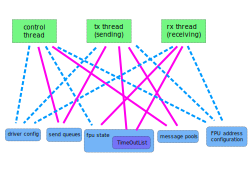
\includegraphics[width=0.9\textwidth]{fpu-driver-concurrency-architecture.png}
\caption{Overview of Concurrency architecture of FPU driver}
\label{fig:overview}
\end{sidewaysfigure}

Figure~\ref{fig:overview} gives an overview on the concurrency
structure in the \texttt{fpu\_driver} module.

\subsection{Threads}

In the top row of the figure we see three rectangles,
which represent the three threads which are active
in the running \texttt{fpu\_driver} module. These are:

\begin{description}
\item[Control thread] The ``control''  thread is identical to the main thread of
  the program. It's functions are entered when new commands are sent
  to the FPUs, and return when the result of the commands is returned
  to the caller. In the time between, the thread could be
  blocked. This works almost exactly as in the same way
  as, for example, a \texttt{read()} or \texttt{write()} library
  call in a program that uses POSIX file IO.


\item[tx thread] The ``tx'' thread performs the sending of commands to
  the fibre positioners, by sending messages over three socket
  connections. Each socket is connected to one EtherCAN gateway. It is
  structured so that it can send messages as fast as possible. If the
  gateways or the FPUs cannot process messages as fast, it waits until
  one of the sockets is writable.

\item[rx thread] The ``rx'' thread reads any return messages from the
  fibre positioners to the driver, and updates the driver's internal
  structures which describe the state of the FPUs. It is designed so
  that it can read messages as fast as possible. Especially, the rx
  thread is designed so that it never has to wait itself for any
  long-running or potentially blocking operation, such as a file read,
  or a network response.

\end{description}


\subsection{Data structures}

The rounded boxes in the bottom of the figure represent the main data
structures which these three threads are accessing.

The arrows show the type of access. There are two types of access,
read-only access, which is symbolised by broken blue arrows, and
modifying access, which is depicted by magenta straight arrows. We see
that there are two data structures which are different, in that they
only receive read-only access. As matters around them are simpler, we
will discuss them first.

\subsubsection{Read-only data}

The read-only data structures are as follows:

\begin{description}
\item[Driver configuration] This structure holds the parameters which
  define the global configuration of the driver, for example the
  minimum motor frequency required in waveforms. It has the type
  \texttt{EtherCANInterfaceConfig}, and is passed as a constant
  argument to the driver's constructor. Because it is in no place
  modified, we know that it does not change, and we can pass it
  everywhere as constant.

\item[FPU address configuration] This structure is a table which maps
  the logical FPU numbers to the address triplet of (gateway number,
  bus number, and CAN ID on the bus). The table is created at program
  start-up, and passed to the threads when they are created.

  Synchronisation of the table poses an interesting question: If the
  table is created at program start-up, it is modified in the control
  thread. After this, the tx thread and the rx thread are created. How
  can we be sure that this modification is not seen in the newly
  created threads?

  The answer to this is that the creation of threads in pthreads
  causes a so-called memory barrier. Any data which was written by the
  CPU before that thread was created, is written to memory before the
  new thread can see it. This is important, because normally in a C
  program with different threads, there is \emph{no} notion of
  ``before'' or ``after'' for operations in different threads, unless
  such operations are explicitly synchronised. The thread creation
  represents such an synchronisation point.



\end{description}

\subsection{Message queues}
Furthermore, we have three main data structures which are not only
read concurrently, but also modified. We discuss the message queues
first.

Message queues are thread-safe data structures which allow the control
thread to send parametric messages for individual FPUs to the tx
thread. The control thread is responsible for setting up the messages
and its actual data content, and the tx thread is responsible for
sending them.

To achieve that, the control thread inserts each message into a data
structure which is basically a thread-safe FIFO or ring buffer.  The
insertion method uses locks to ensure that the internal invariants of
the data structure are kept correct, and that no unsynchronized
concurrent modifications occur. There is one message queue for each
socket. Using the FPU's address configuration, the control thread
knows into which queue to insert a message.

The tx thread checks whether there are messages in the message queues,
\emph{and} whether it can send a message to a socket without blocking
(this is done using the \texttt{epoll()} syscall). If this is the
case, the message is serialized into a byte sequence and written to
the socket; the remaining processing is handled by the OS kernel.

\subsection{Message pools}

One aspect that is missing is what happens with the message after it
was processed by the RX thread. Messages could be values which are
copied. However, it is useful to treat them as object instances which
have virtual methods, which allows some degree of abstraction.

As such objects can have different sizes, they need to be passed by
pointers, and their memory needs to be managed.  This is done by C++
smart pointers (more precisely, \texttt{std::shared\_ptr<>}). In
theory, each message object could be allocated, using \texttt{new},
when it is needed, and deallocated, using \texttt{delete}, when it is
not longer needed. However this is relatively slow. Therefore,
messages are taken from a set of message pools, which are created on
program start-up, and are inserted back into the pool when they are
not needed at the moment.

The resulting pattern is that the control thread takes a message from
a message pool, and inserts it into a message queue. Then, the tx
thread pops it from the message queue, sends its byte representation,
and recycles the message by adding it to the corresponding message
pool. With this scheme, no dynamic allocation of messages is needed
after program start-up, so this is much faster.

As a detail, there is one pool for each type of message, and the pools
are simpler organized than the message queues, they are basically a
stack of smart pointers.

\subsection{FPU state handling}

After looking at the message queues and message queues, we can now
look at the remaining data structure, which is more complex, and very
central to the FPU driver software. It is represented by the larger
rectangular box in the middle, and provides a data structure which
records the FPU's state with each response message that was received
from the gateway. Because we have one such state record for each of
the 1001 FPUs, this structure is called the \texttt{FPU\_state} array.

For the moment, we will temporarily ignore the box which is labelled
``\texttt{TimeOutList}'', it will be explained soon.

The responses messages are received by the rx thread, of course.
Therefore, the rx thread writes the state updates into the FPU state
array, symbolized by the magenta arrow. The control thread reads from
the state array. To avoid corruption by concurrent modification, it
uses a lock or Mutex, which ensures that write accesses and read
accesses are mutually exclusive. The rx thread keeps this lock most of
the time. Only for short moments, the look gets released, which gives
the control thread the opportunity to read back the new state data,
and return it to the caller of the driver method.

\subsection{The \texttt{TimeOutList} data structure}

We promised to have a look at the data structure
\texttt{TimeOutList}, which is written to by both
the tx thread, and the rx thread. Its function is
as follows:

Normally, most messages to an FPU are promptly followed by a response
within a few milliseconds. However, it can happen that this runs into
errors, for example if the connection to the CAN bus gets broken. In
this case, the response will never arrive, and the driver needs to
handle this.

This is done by a sorted list of time-out times. Each time when a
message is sent to an FPU, an expiration time for the message is
computed, and this time is added as a time stamp to the list of time
outs.

Each time when the rx threads starts to wait for a new message, it
looks for the next time-out, and waits at most until this moment. If
the waiting time ends without a response, all FPUs whose time-out time
stamp has expired, are marked as timed out.

To manage time-outs in such a way, the \texttt{TimeOutList} data
structure needs to be modified by both the tx thread and the rx
thread, which is why it is a special component of the FPU state
array. Because it can be modified directly, the \texttt{TimeOutList}
has an own lock, which can be acquired without holding the mutex for
the FPU state array.


\section{Conditional waiting and event messaging}

As outlined above, the methods in the control thread work similar to
system calls like \texttt{read()} or \texttt{write()}, in that they
wait until a driver operation is completed, and return with the
result.

In the case of the \texttt{fpu\_driver}, this means that fairly complex
operations have to complete, because messages are sent to a large set
of 1001 FPUs, and normally we want to wait until each of them has
responded that the command is complete.

Now, this could be implemented in a way that the rx thread holds a
lock on the array for the state of all FPUs, then when a message
arrives, it updates the states, releases the lock, then the control
thread gets the lock, checks whether the operation is complete, if not
it releases the lock, and so on. This has several disadvantages:

\begin{itemize}
\item It is inefficient, because the control thread is not
  really interested in the result for each of the 1000 FPUs individually,
  but rather in the end result of the operation.
\item It is slow, because in the time in which the control thread holds
  the lock, the rx thread cannot do its work and update the
  state with new FPU responses.
\item Its is furthermore quite inefficient, because each time the CPUs
  switch threads, the whole FPU state data structure needs to be
  synchronized between CPU caches, and the OS needs to perform a
  context switch to activate the other thread.
\end{itemize}

To improve on this, pthreads \textbf{condition variables} are used.
Basically, they allow to suspend the control thread until a certain
condition has been reached, which is checked by the rx thread. This
means that the CPU does not need need to switch constantly between the
two threads. Rather, the rx thread has some description of the
specific condition that the control thread waits for, and only if that
condition is probably reached, the control thread is woken up and can
check the state of things.

\subsection{Counters of pending messages}

\subsection{Notification of new commands for the tx thread}

\subsection{Event file descriptors for interrupting epoll()}

\section{A selection of relevant classes and their synchronization objects}

\appendix

\section{Class methods relevant for concurrency}



\end{document}
